%----------------------------------------------------------------------------
\chapter{Háttérismeretek}
\label{chp:background}
%----------------------------------------------------------------------------
Ebben a fejezetben a feladat megértéséhez szükséges technológiákat mutatom be röviden.

%----------------------------------------------------------------------------
\section{Virtuális gépek}
%----------------------------------------------------------------------------
\begin{itemize}
  \item általában egy virtuális gép mire jó
  \item	vagrant szerepe virtuális gépek létrehozásában/konfigurálásában
\end{itemize}

%----------------------------------------------------------------------------
\section{Peer-to-peer fájlátvitel}
\label{sect:p2p}
%----------------------------------------------------------------------------
A Peer-to-Peer(P2P) hálózat olyan, aminek a csomópontjai nem egy kitüntetett géppel 
kommunikálnak, hanem közvetlenül egymással. A klasszikus kliens-szerver és a P2P hálózat felépítését
a~\ref{fig:networkcomparison}~ábra szemlélteti.

\begin{figure}[ht]
	\centering
	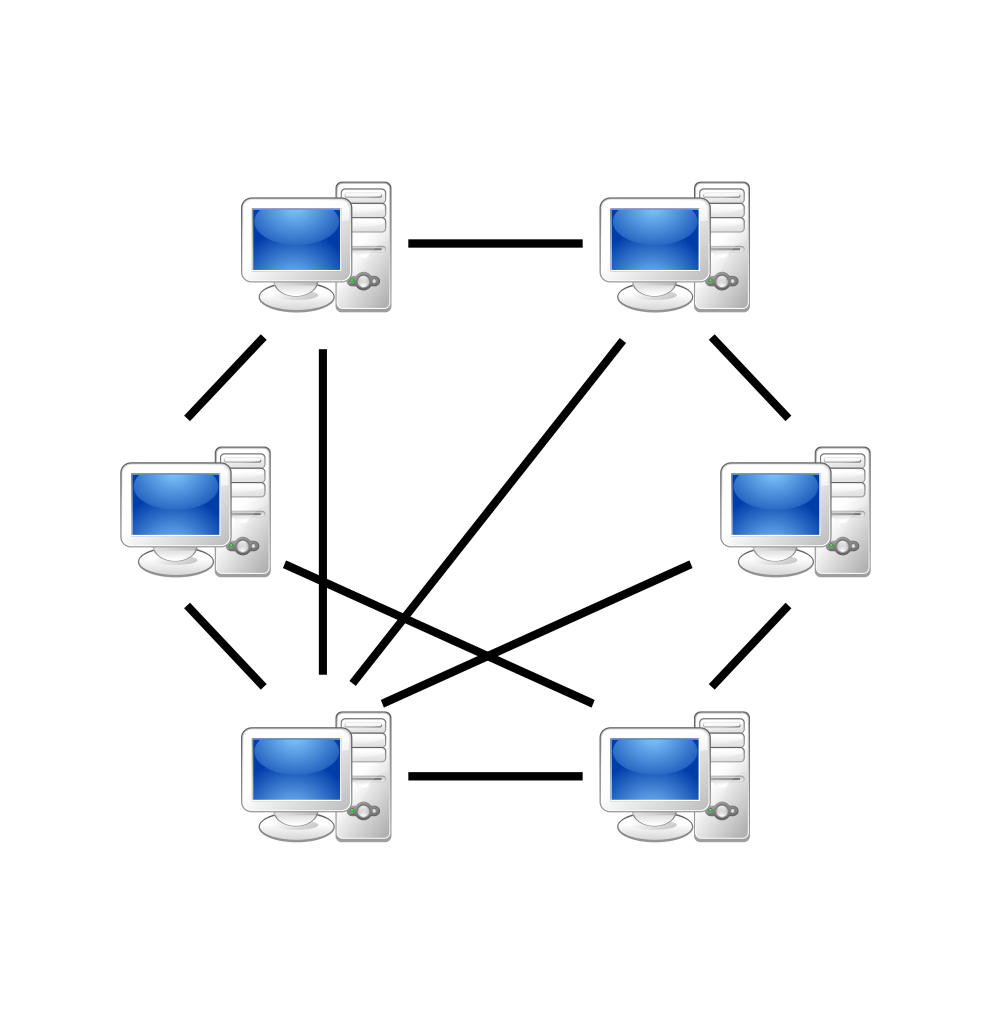
\includegraphics[width=50mm, keepaspectratio]{figures/P2P-network.png}\hspace{1cm}
	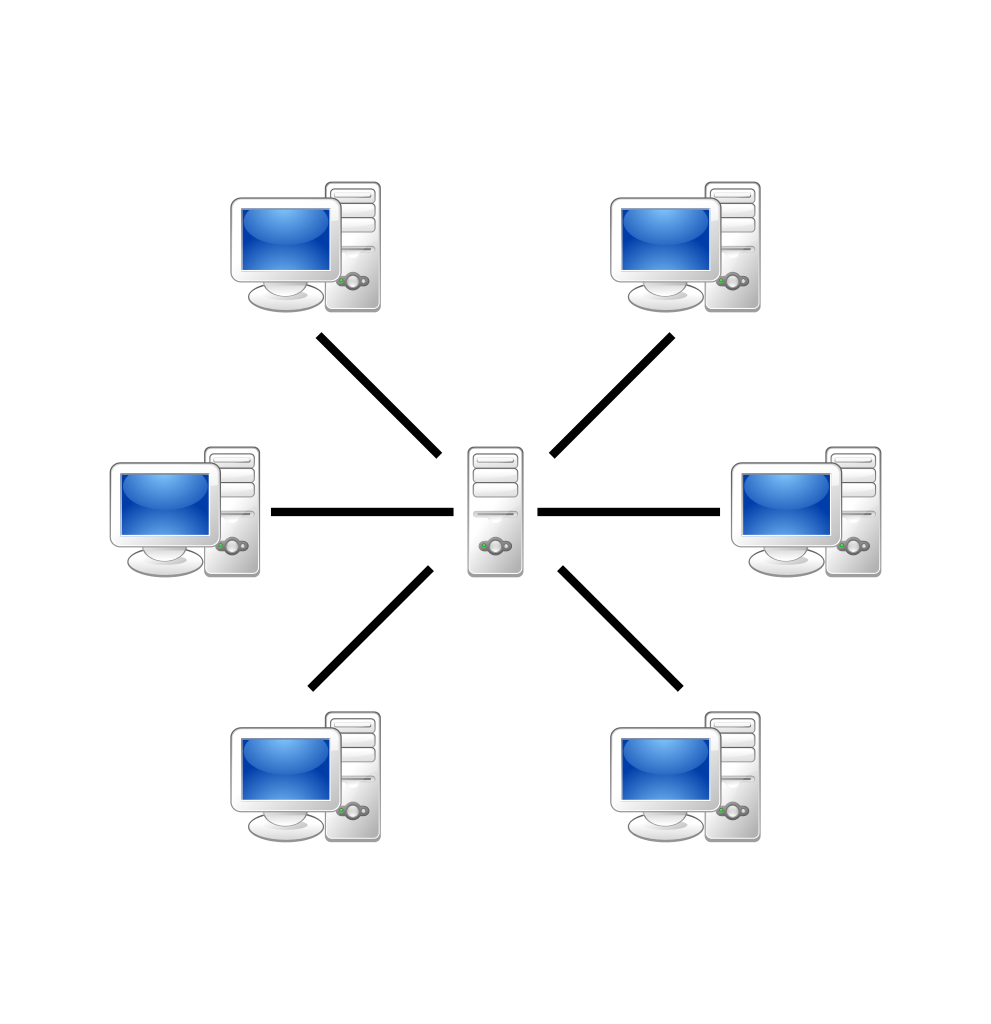
\includegraphics[width=50mm, keepaspectratio]{figures/Server-based-network.png}
	\caption{P2P és kliens-szerver alapú hálózat.}%TODO forrásmegjelölés
	\label{fig:networkcomparison}
\end{figure}

P2P hálózat használatának fő előnye a robusztusság és a skálázhatóság, mivel nincs központi elem,
aminek a meghibásodása szolgáltatáskiesést okozhatna, illetve a hálózat min (például P2P alapú fájlmegosztás esetén esetén a letöltés
mellett fel is tölt). Hátrányai közül a két legjelentősebb a nehezebb karbantarthatóság, és az
esetlegesen fellépő sebességproblémák internetszolgáltató-oldali forgalomkorlátozások miatt.
A P2P alapú technológiák egyik legnagyobb felhasználási területe a tartalomszolgáltatás, ezen belül
az egyik legismertebb ilyen technológiát használó protokoll a Bittorrent. A Bittorrent~\cite{cohen2008bittorrent} protokollt
fájlmegosztásra használjuk, a mögötte álló alapvető ötlet az, hogy a megosztandó fájlokat
feldaraboljuk, és a letöltőknek ezeket a darabokat nem ugyanolyan sorrendben adjuk oda, így ők a
hiányzó darabokat egymástól is tudják tölteni. 

\begin{itemize}
  \item protokoll által használt terminológia bemutatása (seed, tracker, leecher \ldots)
  \item a megoldáshoz használt konkrét alkalmazások rövid leírása (rTorrent, opentracker))
\end{itemize}


%----------------------------------------------------------------------------
\section{Metamodellezés}
%----------------------------------------------------------------------------
\begin{itemize}
  \item modellezés mire jó
  \item	használata hogyan segíthet a feladat megoldásában
  \item eclipse EMF-et használva ez hogyan teljesül
\end{itemize}